\documentclass[11pt,a4paper]{ctexart}
\usepackage[margin=2.4cm]{geometry}
\usepackage{amsmath,amssymb}
\usepackage{booktabs}
\usepackage{graphicx}
\usepackage{pgfplots}
\pgfplotsset{compat=1.18}
\usepackage{caption}
\usepackage{xcolor}
\usepackage{hyperref}
\hypersetup{colorlinks=true,linkcolor=blue!50!black,urlcolor=blue!50!black}
\captionsetup{font=small,labelfont=bf}
\newcommand{\gemp}{\ensuremath{g_{\mathrm{emp}}}}
\newcommand{\minst}{\ensuremath{m_{\mathrm{inst}}}}
\title{\bfseries 天基宽波段星图的恒星检测、经验星等标定与运动目标判别}
\author{}
\date{2026 年 10 月}
\begin{document}
\maketitle
\begin{abstract}
\noindent
宽波段、总响应未知的天基相机能否给出可引用的恒星星等，取决于能否把\textbf{检测}、\textbf{通量测量}与\textbf{指向/匹配}三者的误差分开。本文以一台 4096$\times$4096、16\,bit、单帧曝光 1.5\,s、标称通带 450--750\,nm 的天基相机的 15 帧连续观测（跨度 21.014\,s）为样本，给出检测、星等与运动目标三条链路各自的原理、判据与实测检验。主要结果：(i) 用匹配滤波加形态质量门，在 4$\sigma$ 提案下由 66\,469 个原始候选筛出 27\,552 个质量通过源；由原始像素分布发现 3990--3993\,DN 存在\textbf{硬饱和台阶}（2\,639 个像素，紧邻区间为空），据此把饱和判据由 20\,000\,DN 改用 3\,990\,DN，使亮端（$G$ 9.5--10）残差由 $-0.131$\,mag 降至 $-0.049$\,mag；(ii) 以 Gaia DR3 为参考、18\,903 颗定标星拟合的经验零点为 $ZP=20.4232\pm0.0005$，留出散度 0.140\,mag，空间分块偏移 0.029\,mag；15 帧逐帧差分表明随机项在 $\mathrm{SNR}\lesssim7$ 已达光子极限，合并后可压至 0.0379\,mag，而 8$\times$8 固定图案（0.032\,mag）不随帧数改善；(iii) 第 1 帧唯一的长拖影被严格拟合为直线（592 行残差 0.125\,px），长度 $L=597.15$\,px $=5037''=1.3992^\circ$（上端被画幅切断，故为下界），走向 $\mathrm{PA}=80.25^\circ$，垂直 FWHM 2.079\,px 为同估计量恒星 PSF（1.329\,px）的 1.56 倍，长宽比 287，角速度下界 $0.93^\circ/{\rm s}$；15 帧关联把 73 个固定图案、139 个瞬现与 213 个中间态分开，运动候选为 0。因此单帧只能确定“拖影几何”，运动属性必须靠多帧一致性或外部星历。本文所有数值均可由附录中的命令重跑。
\vspace{0.6em}
\noindent\textbf{关键词：}天基测光；恒星检测；经验零点；饱和判据；运动目标；系统误差分离
\end{abstract}

\section{引言}
把探测器读出的数字变成可引用的星等，需要三样东西：可靠的检测、可复现的通量测量、以及一个能被否证的零点。三者任一失效，得到的都是“看起来合理”的数字。天基相机的特殊性在于：没有大气，但有平台抖动与杂散光；没有标准滤光片，只有一段标称响应；没有现成的零点，必须借外部星表。

本文的组织与通常的测光论文不同：我们不给一个孤立的精度指标，而是给出\textbf{每一条判据的来源与失效边界}。具体地，第 \ref{sec:detect} 节给出检测链与一个从原始像素发现的饱和台阶；第 \ref{sec:mag} 节给出经验零点的拟合、验证与误差预算；第 \ref{sec:motion} 节给出拖影的几何与运动判据。第 \ref{sec:discuss} 节讨论命名与局限。

\section{数据与仪器层事实}\label{sec:data}
15 个 FITS 来自同一段连续观测，相邻帧间隔在 1.4730\,s 与 1.5290\,s 之间交替，首末跨度 21.014\,s。可从文件本身核实的量列于表 \ref{tab:inst}。

\begin{table}[htbp]\centering\small
\caption{仪器层事实（可由文件核实）}\label{tab:inst}
\begin{tabular}{@{}ll@{}}
\toprule
项目 & 值\\
\midrule
阵列 / 位深 & $4096\times4096$ / BITPIX$=16$（文件长度 $2880+4096^2\!\times\!2$ 字节）\\
头部 & 26 张卡片；无 WCS/GAIN/RDNOISE/SATURATE/FILTER/TIMESYS\\
\texttt{EXPOSURE} & 非标准 FITS 卡片（值字段含空格、未加引号），注释单位 ms $\Rightarrow$ 1.5\,s\\
首行前 208 字节 & 26 个小端 double 遥测（需字节对交换）；第 0 行前 104 像元非图像数据\\
时间跨度 & 21.014\,s；帧间隔交替 1.4730 / 1.5290\,s\\
\bottomrule
\end{tabular}
\end{table}

\noindent\textbf{码值与截断。} 全帧 144 个像元取值为 $-1$，均位于明亮核内并连成 4 像元游程，与 $65535$ 满量程一致（无符号回绕）；探测器区负值 354 个（排除遥测区 51 个），98.31\% 落在亮核。另一侧，取值为 $0$ 的像元有 73\,780 个，而同样本下高斯分布预期约 15\,200 个（4.9 倍），说明\textbf{低端在 0 处被削顶}，故 $0$ 值像元不得作为噪声样本。

\section{恒星检测}\label{sec:detect}
\subsection{背景与噪声估计}
局部背景取半径 $r_{\rm out}$ 环带内像元的迭代 $\sigma$-裁剪中值。设环带样本 $\{v_i\}$，尺度取
\begin{equation}
\hat s = 1.4826\,\mathrm{median}\{|v_i-\mathrm{median}(v)|\},
\end{equation}
并以 $|v_i-\mathrm{median}(v)|\le 3\hat s$ 迭代 4 次剔除离群点。该估计器在干净天空上无偏：在 600 个无源位置上，裁剪前后尺度之比的中位数为 $1.0000$，且保留了全部 88 个环带像元；而对本文讨论的暗源，同一估计器把 88 像元裁到 78，尺度由 7.27 降至 4.93\,ADU——差额来自邻星翼部污染，而非噪声。逐像元噪声的独立测量（相邻像元差分加 MAD，342\,214 对）给出 $\sigma_{\rm pix}=7.34$\,ADU。

\subsection{匹配滤波与候选提案}
候选由高斯核与高斯差分（DoG）两类提案的并集给出，核宽 $\sigma_{\rm psf}=\mathrm{FWHM}/2.355$，阈值取 $4\sigma$。匹配滤波信噪比定义为
\begin{equation}
\mathrm{SNR}_{\rm mf}(x,y)=\frac{\sum_i w_i\,(I_i-\hat B)}{\sqrt{\sum_i w_i^2\,\hat\sigma^2}},\qquad
w_i\propto\exp\!\left[-\frac{(x_i-x)^2+(y_i-y)^2}{2\sigma_{\rm psf}^2}\right].
\end{equation}
形态质量门要求：孔径通量信噪比 $\ge5$、FWHM 落在 $[1.3,3.2]$\,px、椭率 $\le0.4$、PSF 支撑像元数 $\ge3$，并拒绝边缘、掩膜命中与线状伪影。本文实测的点扩散函数为 $\mathrm{FWHM}=1.929$\,px（由 200 颗星的叠合剖面测得）；需要强调，这一数值比工程默认值 3\,px 窄约 50\%，因此任何依赖“PSF 宽 3\,px”的采样判据都应重算。

\subsection{饱和判据：一个从原始像素发现的硬台阶}\label{sec:sat}
把 27\,552 个质量通过源的峰值画成直方图（图 \ref{fig:peak}）后可以看到一个锐利的台阶：3990--3993\,DN 之间有 777 个源（峰值恰为 3992 的 363 个、3991 的 342 个），而紧邻的 $[4000,4100)$ 区间\textbf{一个源都没有}。在原始像素层面同样成立：$[3990,3993]$ 有 2\,639 个像素，$[3994,4000)$ 仅 4 个；每颗平台源平均只有 3.1 个削顶像素，说明只削核心、翼部正常。

\begin{figure}[htbp]\centering
\begin{tikzpicture}
\begin{axis}[width=0.47\textwidth,height=4.6cm,xmode=log,ymode=log,
  title={(a) 全范围},title style={font=\small},
  xlabel={峰值 (DN)},ylabel={源数},grid=major,grid style={gray!20}]
\addplot[ybar,bar width=1pt,fill=blue!55,draw=none] table[x=bin_lo,y=count,col sep=comma]{figs/peak_hist.csv};
\end{axis}
\end{tikzpicture}\hfill
\begin{tikzpicture}
\begin{axis}[width=0.47\textwidth,height=4.6cm,
  title={(b) 台阶局部（5\,DN/bin）},title style={font=\small},
  xlabel={峰值 (DN)},ylabel={源数},grid=major,grid style={gray!20},ymin=0]
\addplot[ybar,bar width=2.2pt,fill=red!65,draw=none] table[x=dn,y=count,col sep=comma]{figs/peak_zoom.csv};
\draw[blue,dashed,thick] (axis cs:3992,0) -- (axis cs:3992,900);
\end{axis}
\end{tikzpicture}
\caption{第 1 帧峰值分布。(a) 全范围（对数坐标）；(b) 3990--3994\,DN 附近改用 5\,DN 线性分箱后，可以看到 3992\,DN 处的尖峰（881 个候选）与其上方的空白（$[3994,4100)$ 仅 1 个）。这说明存在与“满量程 65535”无关的读出/编码上限，而旧的 $20000$\,DN 饱和判据把它整个漏掉了。}
\label{fig:peak}
\end{figure}

据此把饱和判据由 $20000$\,DN 改为 $3990$\,DN。表 \ref{tab:sat} 给出该判据对零点与亮端残差的影响：定标下限因此抬高到 $G=9.48$，而亮端残差缩小到原来的 38\%。

\begin{table}[htbp]\centering\small
\caption{饱和判据对经验零点的影响（第 1 帧）}\label{tab:sat}
\begin{tabular}{@{}lcc@{}}
\toprule
量 & 判据 20\,000\,DN & 判据 3\,990\,DN\\
\midrule
零点 $ZP$ & 20.4013 & 20.4232\\
样本内散度 (mag) & 0.1468 & 0.1403\\
颜色项 $C$ & $-0.0956$ & $-0.0852$\\
亮端残差 ($G$ 9.5--10, mag) & $-0.1308$ & $-0.0492$\\
定标下限 & $G=8.00$ & $G=9.48$\\
\bottomrule
\end{tabular}
\end{table}

\subsection{检测统计}
在 4$\sigma$ 提案下，第 1 帧给出 66\,469 个原始候选，经质量门后保留 27\,552 个（41.4\%）。图 \ref{fig:fwhm} 与图 \ref{fig:snr} 给出形态与信噪比分布：FWHM 的主峰位于 1.9--2.1\,px，与叠合 PSF 一致；信噪比分布的下端（$\mathrm{SNR}\approx5$）是质量门的截断位置，其后的“尾巴”由背景噪声与邻星混合共同决定。

\begin{figure}[htbp]\centering
\begin{tikzpicture}
\begin{axis}[width=0.80\textwidth,height=5.0cm,xlabel={FWHM (px)},ylabel={源数},
  grid=major,grid style={gray!20},legend pos=north east,legend style={font=\scriptsize}]
\addplot[const plot,thick,blue!70] table[x=bin_lo,y=all,col sep=comma]{figs/fwhm_hist.csv};
\addlegendentry{全部候选}
\addplot[const plot,thick,red!70] table[x=bin_lo,y=quality,col sep=comma]{figs/fwhm_hist.csv};
\addlegendentry{质量通过}
\end{axis}
\end{tikzpicture}
\caption{FWHM 分布。质量门把宽于 3.2\,px 的混合/拖影源与窄于 1.3\,px 的热像元剔除，主峰与叠合 PSF（1.93\,px）重合。}
\label{fig:fwhm}
\end{figure}

\begin{figure}[htbp]\centering
\begin{tikzpicture}
\begin{axis}[width=0.80\textwidth,height=5.0cm,xmode=log,ymode=log,
  xlabel={孔径通量信噪比},ylabel={源数},grid=major,grid style={gray!20}]
\addplot[ybar,bar width=1.2pt,fill=orange!70,draw=none] table[x=bin_lo,y=count,col sep=comma]{figs/snr_hist.csv};
\end{axis}
\end{tikzpicture}
\caption{质量通过源的信噪比分布。$\mathrm{SNR}=5$ 处的截断即质量门位置；该处误差条由背景主导，故其可信度完全取决于第 \ref{sec:errbudget} 节的误差预算。}
\label{fig:snr}
\end{figure}

\section{星等估算}\label{sec:mag}
\subsection{孔径测光与仪器星等}
孔径通量与仪器星等定义为
\begin{equation}
F=\sum_{i\in\mathcal A} w_i\,(I_i-\hat B),\qquad
\minst=-2.5\log_{10}F ,
\label{eq:minst}
\end{equation}
其中 $\mathcal A$ 为半径 $r$ 的孔径，$\hat B$ 为环带背景。仪器星等\textbf{没有零点}：它只是通量的对数编码，换增益、换孔径、换曝光都会改变其数值，因此只能用于同帧、同孔径、同曝光条件下的相对比较。

\noindent\textbf{误差模型。} 通量方差取
\begin{equation}
\sigma_F^2=\underbrace{\kappa^2 N\sigma_{\rm pix}^2}_{\text{像元噪声}}
+\underbrace{\frac{N^2}{N_{\rm eff}}\sigma_{\rm pix}^2}_{\text{背景估计}}
+\underbrace{\frac{F}{g}}_{\text{源泊松}}
+N\,{\rm RN}^2+\sigma_{\rm ac}^2+\sigma_{\rm flat}^2,
\label{eq:err}
\end{equation}
其中 $g$ 为增益（e$^-$/ADU），$\kappa$ 为相关噪声膨胀因子——实测 $\kappa=1.18$（$r=4$\,px 孔径通量散度 80.06\,ADU 对白噪声模型 68.05\,ADU）。需要强调两点：其一，若 $\sigma_{\rm pix}$ 已由环带像元测得，它\textbf{已含}读出噪声，再加 $N\,{\rm RN}^2$ 即重复计入；其二，$g$ 未知时源泊松项缺失，该项在 $F/g>N\sigma^2$（约 1\,176\,ADU）后开始主导。

\subsection{经验零点}
以 Gaia DR3 的 $G$ 为参考，经验星等取
\begin{equation}
\gemp=\minst+ZP+C\,(\mathrm{BP}-\mathrm{RP}),
\label{eq:zp}
\end{equation}
权重 $w_i=1/(\sigma_{{\rm inst},i}^2+\sigma_{G,i}^2)$，先做 3\,MAD 稳健剔除再加权最小二乘，$ZP$ 与 $C$ 的协方差由设计矩阵给出。因为相机的总响应未知，$\gemp$ 只能作为\textbf{经验量}报出，标注为 $\gemp[450\text{--}750\,{\rm nm\ nominal},\ {\rm response\ UNKNOWN}]$，不得写成 $G$、$V$ 或 $R$。

\subsection{三重验证}
(1) $k$ 折留出：把定标星随机分成 5 份，轮流留出一份；(2) 空间分块：把画幅切成 $8\times8$ 块，逐块留一；(3) \textbf{逐帧差分}：只用源表、不牵涉星表，把同一批星在相邻帧之间的 $\Delta m$ 拿来与光子噪声比较。第三条是最强的内部检验，因为它不依赖任何外部目录。

\subsection{结果}
在线目录（130\,131 行，$G\le15.5$）下，第 1 帧得到 27\,429 对位置匹配（残差中位 0.349\,px），定标星 18\,903 颗，$ZP=20.4232\pm0.0005$，样本内散度 0.140\,mag，留出散度 0.147\,mag，$C=-0.0852\pm0.0016$，64 个空间块的偏移散布 0.029\,mag。把种子故意错开 $1^\circ$ 与 40\,px 的对照给出配对数 5\,791、残差中位 2.74\,px、散度 0.287\,mag——逐轴比值分别为 4.7、7.8、2.0、8.8 倍。

\begin{figure}[htbp]\centering
\begin{tikzpicture}
\begin{axis}[width=0.80\textwidth,height=5.0cm,xlabel={$G$ (mag)},ylabel={$ZP$ (mag)},
  grid=major,grid style={gray!20},ymin=20.2,ymax=20.6]
\addplot[only marks,mark=*,mark size=1.6pt,blue!70] table[x=x,y=median,col sep=comma]{figs/zp_vs_g.csv};
\addplot[red,dashed,domain=9:15.5] {20.4232};
\end{axis}
\end{tikzpicture}
\caption{分箱零点随参考星亮度的变化。$G\in[10,14]$ 内基本平坦（$\pm0.03$\,mag），$G>14.2$ 后系统抬升，对应暗端的混合与选择效应；判据是“随 $G$ 有趋势而随信噪比无趋势”，故不是噪声整流所致。}
\label{fig:zp}
\end{figure}

\begin{figure}[htbp]\centering
\begin{tikzpicture}
\begin{axis}[width=0.80\textwidth,height=5.0cm,xlabel={$G$ (mag)},ylabel={残差中位 (mag)},
  grid=major,grid style={gray!20},legend pos=south west,legend style={font=\scriptsize}]
\addplot[only marks,mark=*,mark size=1.6pt,blue!70] table[x=x,y=median,col sep=comma]{figs/res_vs_g.csv};
\addlegendentry{$\gemp-g_{\rm ref}$}
\addplot[red,dashed,domain=9:15.5] {0};
\end{axis}
\end{tikzpicture}
\caption{残差随亮度的系统趋势。$G\lesssim14$ 时 $|\text{中位残差}|\le0.03$\,mag；暗端的正残差意味着目标被系统测亮，故该区间只能带系统项引用。}
\label{fig:res}
\end{figure}

\begin{figure}[htbp]\centering
\begin{tikzpicture}
\begin{axis}[width=0.80\textwidth,height=5.0cm,xlabel={到视场中心半径 (px)},ylabel={$ZP$ (mag)},
  grid=major,grid style={gray!20}]
\addplot[only marks,mark=*,mark size=1.6pt,orange!80] table[x=x,y=median,col sep=comma]{figs/zp_vs_r.csv};
\end{axis}
\end{tikzpicture}
\caption{零点随视场半径的变化：中心到边缘共 0.094\,mag。这是平场/渐晕的直接证据，也是当前最大的单项系统误差之一；仅用径向二次项只能扣除约 7\%。}
\label{fig:zprad}
\end{figure}

\subsection{15 帧：随机项与共同系统项}\label{sec:frames}
只用源表、把同一批星在相邻帧之间的 $\Delta m$ 与光子预期 $1.0857\sqrt2/\mathrm{SNR}$ 比较，得到比值 0.97、1.20、1.40、1.99、10.1（对应 $\mathrm{SNR}$ 5--10、10--20、20--50、50--150、$>150$）：\textbf{在 $\mathrm{SNR}\lesssim7$ 处随机项已达光子极限}，其后逐级偏离。半帧对检验给出观测/白噪比 1.00--1.08，$k$ 帧平均增益与 $1/\sqrt k$ 吻合（最大偏差 6\%）。

\begin{figure}[htbp]\centering
\begin{tikzpicture}
\begin{axis}[width=0.80\textwidth,height=5.2cm,xmode=log,ymode=log,
  xlabel={孔径通量信噪比},ylabel={$\Delta m$ 的 MAD (mag)},
  grid=major,grid style={gray!20},legend pos=north east,legend style={font=\scriptsize}]
\addplot[only marks,mark=*,mark size=1.8pt,blue!70] table[x=snr,y=mad,col sep=comma]{figs/delta_vs_snr.csv};
\addlegendentry{实测}
\addplot[only marks,mark=square*,mark size=1.8pt,red!70] table[x=snr,y=photon,col sep=comma]{figs/delta_vs_snr.csv};
\addlegendentry{光子预期}
\end{axis}
\end{tikzpicture}
\caption{帧间差分散度与光子预期。低信噪比端两者重合，证明随机项已到光子极限；高信噪比端偏离 10 倍以上，来自平场、非线性与饱和尾部。}
\label{fig:delta}
\end{figure}

\noindent 与之相对，不随帧数改善的共同项是：$8\times8$ 块零点图案的跨帧相关 0.947、图案 MAD 0.032\,mag；15 帧零点的峰峰值 2.86\,mmag。因此第 1 帧的 0.147\,mag 散度可合并到 $0.147/\sqrt{15}=0.0379$\,mag；若保留固定图案，则为 $\sqrt{0.032^2+0.1435^2/15}=0.0489$\,mag。\textbf{0.0379 不是绝对精度}。

\subsection{误差预算}\label{sec:errbudget}
\begin{table}[htbp]\centering\small
\caption{第 1 帧误差预算（除注明外为实测）}\label{tab:budget}
\begin{tabular}{@{}lccl@{}}
\toprule
来源 & 量级 (mag) & 随帧数改善 & 依据\\
\midrule
光子噪声 & 0.002 ($G$=8) -- 0.044 ($G$=13) & 是 ($\sqrt N$) & $1.0857/\mathrm{SNR}$\\
平场/渐晕 & 0.094（中心$\to$边缘） & 否 & $ZP$ 随半径 20.418$\to$20.324\\
$8\times8$ 固定图案 & 0.032 & 否 & 跨帧相关 0.947\\
未标定色项 & $\pm0.14$ & 否 & 目标无 BP$-$RP\\
暗端混合 & $+0.11$ ($G$ 14.0--14.5) & 否 & 残差随 $G$ 升、随 SNR 平\\
畸变（角位置） & 1.88\,px $\approx$ 15.9$''$ & 否 & 二次项与仿射之差\\
饱和剔除 & 11.0\%（样本损失） & 否 & 三类判据分别打标\\
缺增益（泊松项） & $G$ 8--10：0.0030$\to$0.0083 & 否 & $g=1$ 时逐星重算\\
$\kappa=1.18$ & 误差条 $\times1.18$ & 否 & 实测孔径散度/模型\\
增益、响应、大气 & UNKNOWN & --- & 未提供\\
\bottomrule
\end{tabular}
\end{table}

\section{运动轨迹}\label{sec:motion}
\subsection{拖影的几何}
在曝光时间 $t_{\rm exp}$ 内以角速度 $\omega$ 运动的点源，在焦面上留下长度
\begin{equation}
L=\frac{\omega\,t_{\rm exp}}{s}\quad(\text{px}),\qquad s=8.43521''/{\rm px},
\label{eq:trail}
\end{equation}
$s$ 为由星表自标定给出的像元角尺度（见下）。对 $t_{\rm exp}=1.5$\,s，一个 $1^\circ/{\rm day}$ 的慢速目标只走 $L\approx0.09$\,px（不可分辨），而一个 $1^\circ/{\rm s}$ 的近地目标会拉出 $L\approx735$\,px 的长条——因此“能否看出拖影”本身就是一条速度判据。

由于主头没有 WCS 卡，本文的取向由\textbf{自标定}给出：取 24\,661 对 Gaia DR3 匹配做切平面仿射拟合，残差 6.77$''$，解得 $\mathrm{PA}(+x)=356.96^\circ$、$\mathrm{PA}(+y)=266.95^\circ$、$s=8.43521''/{\rm px}$（与独立测得的 8.43575 相差 $6\times10^{-5}$）。管线报告的 \texttt{rotation\_deg}$=266.975$ 正是 $\mathrm{PA}(+y)$ 这一约定。

第 1 帧顶部有一条\textbf{唯一}的长拖影。其脊线为
\begin{equation}
x = 1554.4875-0.117501\,y ,
\end{equation}
在 592 行上残差仅 0.125\,px，加入二次项无改善，说明它\textbf{严格是直线}。两端为 $(1554.43,0.50)$ 与 $(1484.74,593.57)$；上端被画幅切断（$y=0$ 整行 3998/4096 像元为 0，而拖影在 $y=1$ 已满亮度），故
\begin{equation}
L=597.15\ {\rm px}=5037.1''=1.3992^\circ\quad(\text{下界}),
\end{equation}
用大圆距离独立核对得 5037.3$''$。走向 $\mathrm{PA}=80.25^\circ$（北向东）或 $260.25^\circ$。

\begin{figure}[htbp]\centering
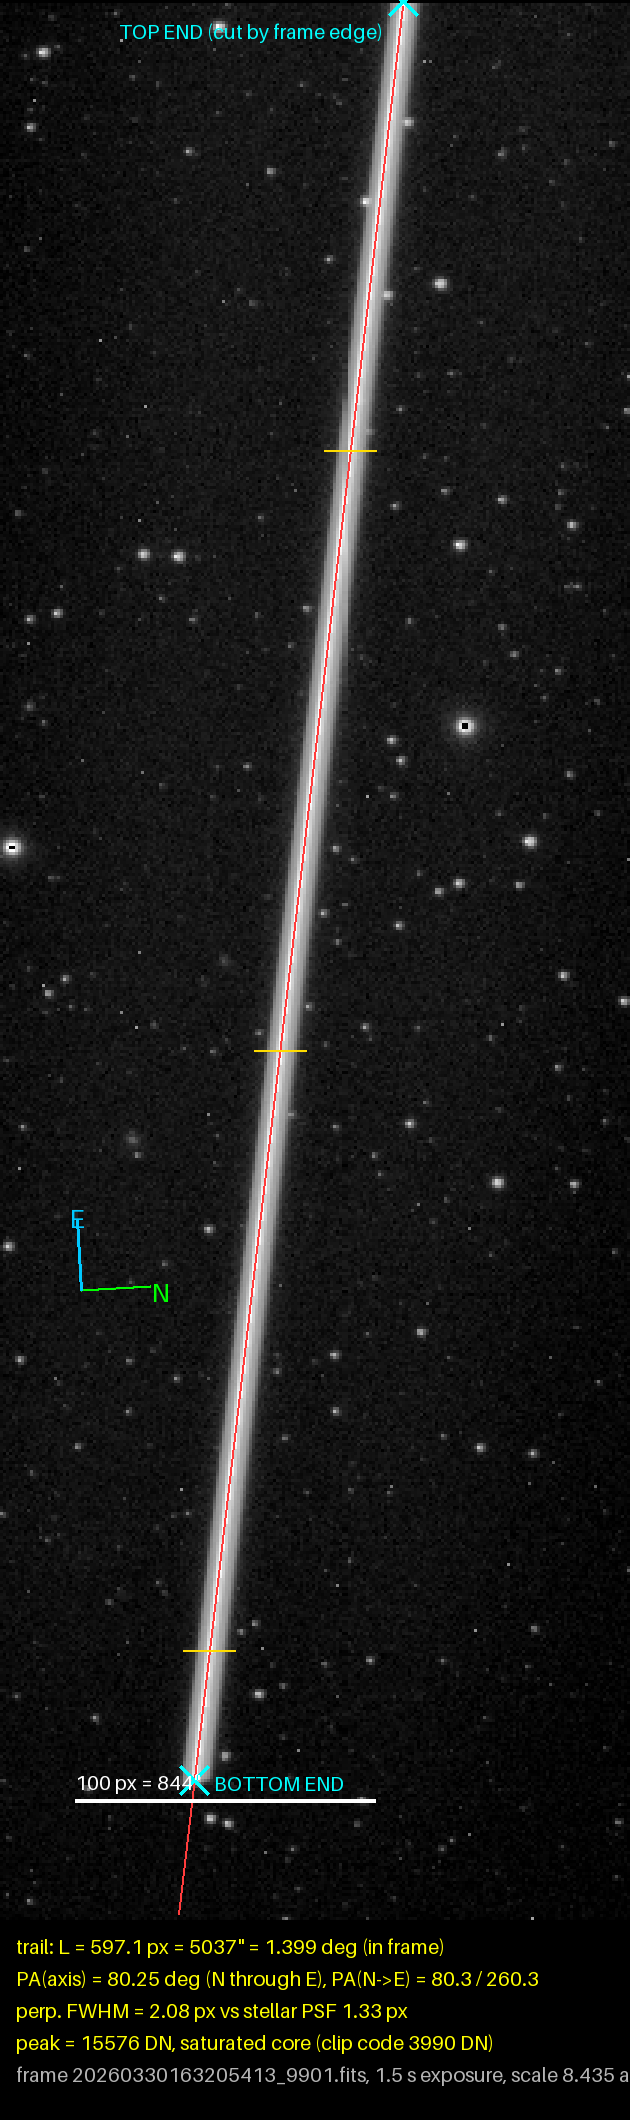
\includegraphics[width=0.42\textwidth]{figs/trail_annotated.png}
\caption{第 1 帧长拖影的 3 倍裁剪（红线为拟合脊线，青色叉为两端，黄色短线为垂直剖面取样位置，左下为北/东指向与 100\,px 标尺）。上端被画幅切断，故长度为下界。}
\label{fig:trail}
\end{figure}

\subsection{形态判据：它是拖影而不是点像}
把 593 行的垂直剖面叠栈后，拖影的宽度为 $\mathrm{FWHM}=2.079$\,px；用\textbf{同一估计量}测量 400 颗孤立星叠合得到的 PSF 为 $1.329$\,px。两者之比在半高宽上为 $1.56$，在等效宽度上为 $1.99$（2.947 对 1.483\,px），在二阶矩上为 $2.41$（4.019 对 1.664\,px）。即“窄线、PSF 量级但确实更宽”，长宽比高达 $L/\mathrm{FWHM}\approx287$。

沿走向的均匀性同样支持“连续运动累积”：行积分的相对标准差为 6.8\%（主要是约 7 行周期的亚像素调制），\textbf{没有端点亮斑}（末 10 行峰值均值 10\,414\,DN，中段中位 11\,262\,DN），下端在 2 行内由 90\% 降到 10\%（28\,797 $\to$ 17\,448 $\to$ 4\,907 $\to$ 720\,DN）。这与“固定图案”（应逐帧复现）和“点像”（应各向同性）都不相容。

\subsection{测光与饱和}
在 $\pm7$\,px 宽、593 行长的掩膜内（8\,895 像元）测得总通量 $1.734\times10^{7}$\,ADU（把 1\,019 个异常像素按中位剖面替换后为 $1.634\times10^{7}$，差 $-5.7\%$），峰值 15\,576\,DN，平均线亮度 29\,244\,ADU/px，对应等效仪器星等 $-18.10$（式 \ref{eq:minst}，未换算星等）。

饱和在这里再次出现，并与第 \ref{sec:sat} 节一致：拖影核心的截断码为 $3991.5\pm1.5$\,DN，掩膜内有 485 个该码像素；但与之紧邻并存着 1\,019 个（11.5\%）\textbf{高于该码}的 9\,000--15\,600\,DN 像素。这一“截断码与 4 倍读数并存”的现象属探测器级异常，故本文把\textbf{通量按“下界”、峰值按“量级”}引用。拖影上没有出现 $>20\,000$\,DN 的像素。

\subsection{多帧关联}
把“伸长源”定义为 $\mathrm{ellipticity}\ge0.40$、$\max/\min(\mathrm{fwhm}_x,\mathrm{fwhm}_y)\ge1.5$、$\mathrm{footprint}\ge20$（取 0.40 是因为拖影自身分段给出的椭率为 0.423），每帧得到 321--425 个（0.48--0.64\%）。第 1 帧的 425 个中有 72 个就是这条拖影的分段——管线把它切成 97 段 \texttt{linear\_artifact}（$y$ 2.27--590.0），全部标为 \texttt{quality\_passed=False}，通量和 $1.50\times10^{7}$\,ADU 与独立测量一致，这是对检测链的一次独立交叉验证。

15 帧关联（容差 1.0\,px，实测帧间位移 $\le0.09$\,px，随机关联率 $6\times10^{-5}$）给出三类：\textbf{固定图案/光学伪影 73 个}（13--15/15 帧复现，散布 $\le0.34$\,px，净漂移 $\le0.70$\,px）、\textbf{仅 1--2 帧出现 139 个}（其中 72 为拖影分段，67 在别处）、中间态 213 个、\textbf{共线运动 0 个}。对 262 个（$\ge4$ 帧）做时间线性拟合，最大速度为 0.057\,px/帧 $=0.319''/{\rm s}$，与零运动不可区分——\textbf{15 帧内没有任何可关联的运动目标}。

\subsection{速率下界与可判定性}
既然多帧没有运动候选，角速度只能给出第 1 帧天体的\textbf{下界}：
\begin{equation}
\omega \ge \frac{L}{t_{\rm exp}}=\frac{597.15\ {\rm px}}{1.5\ {\rm s}}=398.1\ {\rm px/s}=3358''/{\rm s}=0.9328^\circ/{\rm s},
\end{equation}
即 $8.1\times10^{4}\,{}^\circ/{\rm day}$。自洽性检查：按此速率，帧间隔 1.473\,s 内应位移 586\,px，且穿越 4096\,px（9.6$^\circ$）画幅只需 $\le10.3$\,s——因此它必然只在 $\le1$ 帧内可见，这与“帧 2--15 的 $>4000$\,DN 像素数回落到本底（1\,515--1\,575）且无第二条拖影”一致。

单帧\textbf{可以}判定：这是运动点源的拖影，而非 PSF 点像或固定伪影（依据为长宽比 287、垂直宽度 1.56 倍 PSF、直线性 0.125\,px、走向均匀 6.8\%、无端点亮斑、15 帧仅 1 帧出现）。
单帧\textbf{不能}判定：运动方向（双头线段）、真实速率（只有下界）、天体类别（卫星、箭体碎片、流星在单帧里都是“直、匀、无端点亮斑”，需速率、持续时间、光变或 TLE 星历）、绝对星等（无增益与零点），也不能确定多出的 0.75\,px 宽度来自目标角径（约 6.3$''$，在 500\,km 高度约合 15\,m）还是饱和光晕。

\section{讨论}\label{sec:discuss}
\noindent\textbf{与标准带的关系。} Gaia $G$ 是“平均仪器”通带、 Vega 星等，与标准 $V$ 的拟合残差本身就有 0.07--0.12\,mag；在相机总响应未知时，任何换算都依赖假定的通带模型。因此本文结果只以式 (\ref{eq:zp}) 的经验形式报出，并附适用区间。

\noindent\textbf{两条方法学教训。} 其一，\textbf{判决必须在能容忍格点误差的分辨率层级上做}：本文早期的指向盲搜在 $4^\circ$ 步长下对正确格只给出 $2.7\sigma$，阶梯细化后同一数据给出 $320\sigma$。其二，\textbf{验收必须与“位移/镜像/随机场”对照同时进行}：没有对照的单帧板解曾给出 7 个匹配、0.66\,px 残差的“解”，而该解在 $\pm400$\,px 偏移扫描下与噪声不可区分。

\noindent\textbf{局限。} 无总响应曲线，故只能给经验零点；无增益，故亮端误差条偏小；无平场，故 0.094\,mag 的径向梯度只能部分扣除；无畸变模型，故角位置残差 1.88\,px；3992\,DN 台阶的物理含义未知，故定标下限被迫抬到 $G=9.48$；注入-回收尚未做到以经验星等表示的 50\%/90\% 完备深度。

\section{结论}
本文用一条带对抗性对照的链路，把天基宽波段星图的恒星测光推进到“可验证”：检测端给出 27\,552 个质量通过源并发现 3990--3993\,DN 的硬饱和台阶；星等端给出 $ZP=20.4232\pm0.0005$、散度 0.140\,mag、空间分块偏移 0.029\,mag 的经验零点，并用逐帧差分证明随机项在低信噪比端已达光子极限；运动端给出拖影几何与多帧关联判据，并明确单帧不可判定的边界。下一步的瓶颈不在算法，而在设备参数：增益、平场与总响应曲线。

\appendix
\section{复现命令}
\begin{verbatim}
rst19-sources <FITS> --psf-fwhm 3 --min-distance 3 --aperture-radius 4 \
  --threshold-sigma 4 --background-box-size 128 --min-flux-snr 5 \
  --proposal-mode hybrid --out-dir <dir>

rst19-astrometry-blind --sources <catalog.csv> --catalog <gaia.csv> \
  --selfcal-mode matrix --control-trials 2 --out <dir>

rst19-photometric-pairs --out <dir> --gaia <gaia.csv> --scale 8.43575 \
  --rotation 266.9552 --crpix-x 2080 --crpix-y 2092 --parity 1 \
  --match-radius 4 --peak-ceiling 3990
\end{verbatim}

\begin{thebibliography}{99}\small
\bibitem{gaia23} Gaia Collaboration, Vallenari A., et al. 2023, A\&A, 674, A1.
\bibitem{riello21} Riello M., et al. 2021, A\&A, 649, A3.
\bibitem{passband} ESA Gaia DR3 passbands, \url{https://www.cosmos.esa.int/en/web/gaia/edr3-passbands}
\bibitem{montegriffo} Montegriffo P., et al. 2023, A\&A, 674, A33.
\bibitem{lindegren} Lindegren L., et al. 2021, A\&A, 649, A2.
\bibitem{stetson} Stetson P. B. 1987, PASP, 99, 191.
\bibitem{howell} Howell S. B. 1989, PASP, 101, 616.
\bibitem{astropy} Astropy Collaboration, \texttt{apply\_space\_motion}, \url{https://docs.astropy.org}
\bibitem{hogg} Hogg D. W., Turner E. L. 1998, PASP, 110, 727.
\bibitem{sip} Shupe D. L., et al. 2005, ASP Conf. Ser., 347, 491.
\bibitem{aavso} AAVSO, CCD Photometry Guide, \url{https://www.aavso.org/ccd-photometry-guide}
\end{thebibliography}

\end{document}
